\chapter{Reti di Petri}
\section{Introduzione}
Le reti di Petri è un sistema a transizione di stati che estende la classe delle reti elementari.
\begin{defn}
    Una \textbf{rete} è una tripla $N = (B, E, F)$ tale che:
    \begin{itemize}
        \item $B$ è un insieme finito di \textbf{stati locali} \footnote{Con stati locali si intende lo stato di una parte del sistema che si vuole rappresentare. Lo stato globale farà invece riferimento a tutto il sistema.}.\\
        Uno stato locale può essere visto come una condizione sul sistema che si vuole rappresentare.
        \item $E$ è un insieme finito di \textbf{eventi}, detti anche transizioni locali.
        \item $F$ è una \textbf{relazione di flusso}, ovvero la relazione che collega stati locali con eventi ed eventi con stati locali \footnote{Si può osservare che una rete definisce un grafo bipartito, dove i due sottoinsiemi che definiscono la partizione sono $B$ ed $E$.}.
        \[
            F \subseteq (B \times E) \cup (E \times B)
        \]
        Per definizione, inoltre, ogni evento della rete ha almeno uno stato locale di ingresso e almeno uno stato locale di uscita.
        \[
            \forall e \in E, \exists p, q \in B : (p, e) \in F \land (e, q) \in F.
        \]
    \end{itemize}
\end{defn}

Graficamente, gli elementi di una rete di Petri sono rappresentati come:
\begin{itemize}
    \item stato locale falso: $\fPlace$
    \item stato locale vero: $\tPlace$
    \item evento: $\event$
    \item transizione: $\longrightarrow$
\end{itemize}

\begin{defn}
    Dato un elemento $x \in B \cup E$, è possibile definire i due seguenti insiemi:
    \begin{align*}
        \preCond{x} &= \cbra{y \in B \cup E : (y, x) \in F}\\
        \postCond{x} &= \cbra{y \in B \cup E : (x, y) \in F}
    \end{align*}
    Se $x$ è un evento, allora $\preCond{x}$ sono le \textbf{pre-condizioni} di $x$, mentre $\postCond{x}$ sono le \textbf{post-condizioni} di $x$.\\
    Se invece $x$ è uno stato locale, $\preCond{x}$ sono i \textbf{pre-eventi} di $x$, mentre $\postCond{x}$ sono i \textbf{post-eventi} di $x$.
    
    \upperAccE possibile estendere la definizione di questi due insiemi anche a insiemi di stati locali ed eventi. Sia $X \subseteq B \cup E$, allora:
    \begin{align*}
        \preCond{X} &= \bigcup\limits_{x \in X} \preCond{x}\\
        \postCond{X} &= \bigcup\limits_{x \in X} \postCond{x}
    \end{align*}
\end{defn}

\begin{defn}
    Una rete è \textbf{semplice} sse:
    \[
        \forall x, y \in B \cup E, \preCond{x} = \preCond{y} \land \postCond{x} = \postCond{y} \rightarrow x = y
    \]
    \begin{marginfigure}[-5cm]
        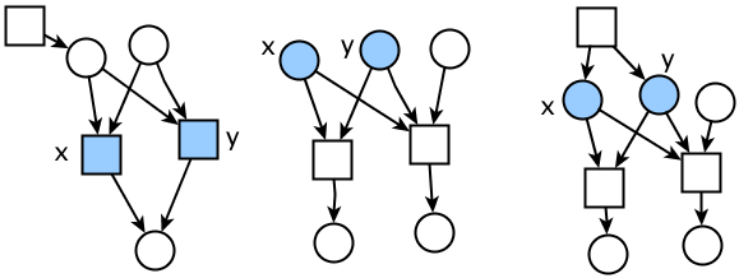
\includegraphics[width=1\linewidth]{images/reti_non_semplici.png}
        \caption{Reti non semplici}
        \label{fig:reti_non_semplici}
    \end{marginfigure}
\end{defn}

\begin{defn}
    Una rete è \textbf{pura} sse:
    \[
        \forall e \in E, \preCond{e} \cap \postCond{e} = \emptyset
    \]
    \begin{marginfigure}[-1cm]
        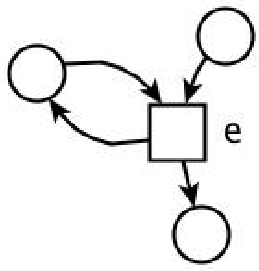
\includegraphics[width=0.4\linewidth]{images/rete_non_pura.png}
        \caption{Rete non pura.}
        \label{fig:rete_non_pura}
    \end{marginfigure}
\end{defn}

\begin{defn}
    Una \textbf{configurazione} della rete è un sottoinsieme di stati locali, $c \subseteq B$.

    Una configurazione rappresenta tutte le condizioni vere per l'intero sistema in un certo istante. Di conseguenza, una configurazione definisce uno stato globale del sistema.
\end{defn}

\begin{defn}
    Una \textbf{rete elementare} \footnote{Una rete elementare viene anche chiamata sistema elementare.} è una coppia $(N, c)$, dove $N$ è una rete e $c$ è la configurazione iniziale per la rete $N$.
\end{defn}

\begin{defn}
    Un evento $e$ è \textbf{abilitato} in una rete $N$ per la configurazione corrente $c$ sse:
    \[
        \preCond{e} \subseteq c \land \postCond{e} \cap c = \emptyset
    \]
    ovvero tutte le sue pre-condizioni sono vere, mentre tutte le sue post-condizioni sono false.\\
    METTERE TRE IMMAGINI. UNA EVENTO ABILITATO, UNA NON ABILITATO PER PRE COND E UNA NON ABILITATO PER POST COND\\
    La configurazione del sistema dopo aver eseguito $e$, indicata con $c'$, sarà:
    \[
        c' = \bra{c \setminus \preCond{e}} \cup \postCond{e}
    \]
    L'occorrenza di un evento $e$ nella configurazione corrente $c$ che porta alla configurazione $c'$ viene indicata con $\canFire{c}{e}{c'}$.
\end{defn}

\begin{defn}
    Un insieme di eventi $U \subseteq E$ è un \textbf{passo} sse tutti i suoi eventi sono indipendenti, ovvero eventi diversi di $U$ non condividono alcuno stato locale.
    \[
        \forall e_1, e_2 \in U, e_1 \neq e_2 \rightarrow (\preCond{e_1} \cup \postCond{e_1}) \cap (\preCond{e_2} \cup \postCond{e_2}) = \emptyset
    \]
\end{defn}

\begin{defn}
    Un insieme di eventi $U \subseteq E$ è un \textbf{passo abilitato} per la configurazione corrente $c$ sse:
    \[
        U \tn{ è un passo } \land \forall e \in U, \canFire{c}{e}{}
    \]
\end{defn}

\begin{defn}
    L'\textbf{insieme delle configurazioni raggiungibili} $C_{\Sigma} \subseteq 2^{B}$ dal sistema elementare $\Sigma = (B, E, F, c_{\tn{start}})$ definito come:
    \begin{itemize}
        \item $c_{\tn{start}} \in C_{\Sigma}$
        \item $\bra{c \in C_{\Sigma} \land \exists U \subseteq E : \canFire{c}{U}{c'}} \rightarrow c' \in C_{\Sigma}$
    \end{itemize}
\end{defn}

\begin{defn}
    L'\textbf{insieme dei passi} $U_{\Sigma}$ di un sistema elementare $\Sigma$ sono tutti i passi possibili che il sistema $\Sigma$ può compiere.
    \[
        U_{\Sigma} = \cbra{U \subseteq E \, | \, \exists c_1, c_2 \in C_{\Sigma} : \canFire{c_1}{U}{c_2}}
    \]
\end{defn}

\begin{defn}
    Siano $N_1 = (B_1, E_1, F_1)$ e $N_2 = (B_2, E_2, F_2)$ due sistemi elementari, $N_2$ è \textbf{sottorete} di $N_1$ sse:
    \begin{itemize}
        \item $B_2 \subseteq B_1$
        \item $E_2 \subseteq E_1$
        \item $F_2 = F_1 \cap \bra{\bra{B_2 \times E_2} \cup \bra{E_2 \times B_2}}$
    \end{itemize}
\end{defn}

\begin{defn}
    Sia $N = (B, E, F)$ una rete, la \textbf{sottorete generata da un sottoinsieme di stati locali} $B_1 \subseteq B$ è la rete $N_1 = (B_1, E_1, F_1)$ con:
    \begin{itemize}
        \item $E_1 = \preCond{B_1} \cup \postCond{B_1}$
        \item $F_1 = F \cap \bra{\bra{B_1 \times E_1} \cup \bra{E_1 \times B_1}}$
    \end{itemize}
\end{defn}

\begin{defn}
    Sia $N = (B, E, F)$ una rete, la \textbf{sottorete generata da un sottoinsieme di eventi} $E_1 \subseteq E$ è la rete $N_1 = (B_1, E_1, F_1)$ con:
    \begin{itemize}
        \item $B_1 = \preCond{E_1} \cup \postCond{E_1}$
        \item $F_1 = F \cap \bra{\bra{B_1 \times E_1} \cup \bra{E_1 \times B_1}}$
    \end{itemize}
\end{defn}

\section{Grafo dei casi}
Il comportamento di un sistema elementare $\Sigma = (N, c_{\tn{start}})$ può essere descritto completamente con un grafo dei casi, in cui ogni nodo rappresenta una delle possibili configurazioni di $N$ e ogni arco $(c_i, c_j)$ etichettato con $U$ rappresenta l'esecuzione $\canFire{c_i}{U}{c_j}$ di un passo abilitato $U$ per $c_i$. Essendo un arco etichettato con un passo abilitato del sistema, il grafo dei casi $CG_{\Sigma}$ descrive la \textbf{step semantics} del sistema elementare $\Sigma$.

\begin{defn}
    Il grafo dei casi $CG_{\Sigma}$ di un sistema elementare $\Sigma$ è formalmente definito come la quadrupla $(C_{\Sigma}, U_{\Sigma}, A, c_{\tn{start}})$ dove:
    \begin{itemize}
        \item $C_{\Sigma}$, l'insieme dei casi raggiungibili, è l'insieme dei nodi.
        \item $U_{\Sigma}$, l'insieme dei passi, è l'alfabeto del grafo.
        \item $A = \cbra{(c, U, c') \, | \, c, c' \in C_{\Sigma} \land U \in U_{\Sigma} \land \canFire{c}{U}{c'}}$ è l'insieme degli archi \footnote{Ogni arco è quindi etichettato con un \textit{passo}, ovvero con un insieme di eventi del sistema $\Sigma$.}.
        \item $c_{\tn{start}}$ è la configurazione di partenza.
    \end{itemize}
\end{defn}

\begin{property}
    Il grafo dei casi gode della \textbf{diamond property}.\\
    Se un grafo dei casi $CG_{\Sigma}$ per un sistema elementare $\Sigma = (C_{\Sigma}, U_{\Sigma}, A, c_{\tn{start}})$ presenta gli archi $(c_1, U_1, c_2)$, $(c_2, U_2, c_3)$ e $(c_1, U_2, c_4)$, con $c_1, c_2, c_3, c_4 \in C_{\Sigma} \land U_1, U_2 \in U_{\Sigma} \land U_1 \cap U_2 = \emptyset$,\\
    allora sicuramente il sistema $\Sigma$ ammetterà i passi $(c_4, U_1, c_3)$ e $(c_1, U_1 \cup U_2, c_3)$.
    \begin{marginfigure}[1cm]
        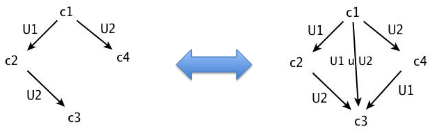
\includegraphics[width=1.05\linewidth]{images/diamond_property.png}
        \caption{Diamond property.}
        \label{fig:diamond_property}
    \end{marginfigure}
\end{property}
La step semantics, e quindi il grafo dei casi, ammette la concorrenza, ovvero ammette archi che rappresentano l'esecuzione concorrente (o parallela?) di almeno due eventi per la configurazione di partenza dell'arco.\\
\upperAccE però possibile definire il comportamento del sistema $\Sigma$ descrivendo le sole sequenze di eventi possibili nel sistema, senza specificare quali eventi possono essere eseguiti in maniera concorrente. Questo tipo di semantica viene detta \textbf{interleaving}, e altro non è che una simulazione sequenziale non deterministica del sistema. La semantica a interleaving di un sistema elementare $\Sigma$ viene descritta tramite il grafo dei casi sequenziale $SCG_{\Sigma}$.

\begin{marginfigure}
    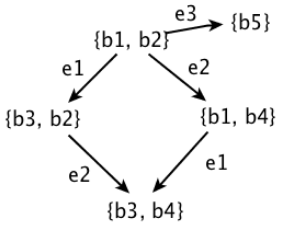
\includegraphics[width=0.60\linewidth]{images/grafo_casi_sequenziale.png}
    \caption{Grafo dei casi sequenziale.}
    \label{fig:sequential_case_graph}
\end{marginfigure}

\begin{defn}
    Il \textbf{grafo dei casi sequenziale} $SCG_{\Sigma}$ di un sistema elementare $\Sigma$ è una quadrapla $(C_{\Sigma}, E, A, c_{\tn{start}})$ dove:
    \begin{itemize}
        \item $C_{\Sigma}$, l'insieme dei casi raggiungibili, è l'insieme dei nodi.
        \item $E$, l'insieme degli eventi, è l'alfabeto del grafo con cui verranno etichettati gli archi.
        \item $A = \cbra{(c, e, c') \, | \, c, c' \in C_{\Sigma} \land e \in E \land \canFire{c}{e}{c'}}$ è l'insieme degli archi \footnote{Ogni arco è quindi etichettato con un \textit{singolo} evento del sistema $\Sigma$.}.
        \item $c_{\tn{start}}$ è la configurazione di partenza.
    \end{itemize}
\end{defn}

\begin{property}
    Il grafo dei casi $CG_{\Sigma}$ e il grafo dei casi sequenziale $SCG_{\Sigma}$ dello stesso sistema elementare $\Sigma$ sono \textbf{sintatticamente equivalenti}, ovvero è possibile ottenere uno a partire dall'altro usando solo procedimenti di modifica sintattica.\\
    MAGARI METTERE ESEMPIO
\end{property}

\begin{thm}
    Due sistemi di transizioni etichettati \footnote{Le reti di Petri sono sistemi di transizioni etichettati.} $A_1 = (S_1, E_1, T_1, s_1)$ e $A_2 = (S_2, E_2, T_2, s_2)$ sono \textbf{isomorfi} sse $\exists \alpha: S_1 \rightarrow S_2 \land \exists \beta: E_1 \rightarrow E_2$ funzioni biunivoche tali che:
    \begin{itemize}
        \item $\alpha(s_1) = s_2$, ovvero la configurazione di partenza di $S_1$ viene mappata nella configurazione di partenza di $S_2$;
        \item $\forall s_i, s_j \in S_1 \land \forall e \in E_1, \quad (s_i, e, s_j) \in T_1 \leftrightarrow (\alpha(s_i), \beta(e), \alpha(s_j)) \in T_2$.
    \end{itemize}
\end{thm}

\begin{rem}
    Due sistemi elementari $\Sigma_1$ e $\Sigma_2$ sono quindi equivalenti sse i loro grafi dei casi (e di conseguenza anche i loro grafi dei casi sequenziali, in quanto sintatticamente equivalenti) sono isomorfi.
\end{rem}

\section{Situazioni particolari}
\subsubsection{Contatto}
\begin{defn}
    Siano $\Sigma = (B, E, F, c_{\tn{start}})$ un sistema elementare, $e \in E$ un evento e $c \in C_{\Sigma}$ una possibile configurazione di $\Sigma$, $(e, c)$ è un \textbf{contatto} sse:
    \[
        \preCond{e} \subseteq c \land \postCond{e} \cap c \neq \emptyset
    \]
    ovvero tutte le pre-condizioni di $e$ sono vere, ma almeno una post-condizione di $e$ è vera.\\
    Un evento che si trova in uno stato di contatto non è abilitato.
\end{defn}

\begin{rem}
    Un evento senza precondizioni è sicuramente un contatto: viene infatti eseguito subito, in quanto l'insieme vuoto delle precondizioni è sempre vero, e quindi le post-condizioni diventano vere. Ma poi l'evento, non avendo pre-condizioni, avrà sicuramente le pre-condizioni vere e tutte le post-condizioni vere. Di conseguenza si ha un contatto. 
\end{rem}

\begin{defn}
    Un sistema elementare $\Sigma = (B, E, F, c_{\tn{start}})$ è un \textbf{sistema senza contatti} sse:
    \[
        \forall e \in E, \forall c \in C_{\Sigma} \quad \preCond{e} \subseteq c \rightarrow \postCond{e} \cap c = \emptyset
    \]
    ovvero se, qualunque sia la configurazione del sistema, le pre-condizione di un evento sono vere, allora sicuramente tutte le sue post-condizioni sono false, e l'evento è abilitato \footnote{In un sistema elementare senza contatti, per stabilire se un evento è abilitato non è necessario effettuare alcun controllo sulle post-condizioni: se le pre-condizioni sono vere, infatti, le post-condizioni saranno sicuramente false.}.
\end{defn}

\begin{rem}
    Ogni sistema elementare $\Sigma$ con contatti può essere trasformato in un sistema elementare $\Sigma'$ senza contatti e con grafo dei casi isomorfo.\\
    Per farlo, per ogni stato $s$ che può essere contatto deve essere aggiunto uno stato complementare $\overline{s}$, vero solo quando $s$ è falso. 
\end{rem}

\begin{marginfigure}[-10cm]
    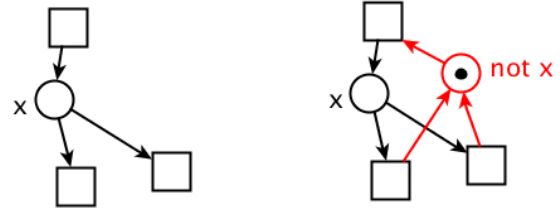
\includegraphics[width=1\linewidth]{images/contatto_complementare.png}
    \caption{Rimozione di un contatto tramite l'aggiunta dello stato complementare.}
    \label{fig:sistema_con_contatti}
\end{marginfigure}

\subsubsection{Conflitto}
\begin{defn}
    Siano $\Sigma = (B, E, F, c_{\tn{start}})$ un sistema elementare, $e_1, e_2 \in E$ due evento e $c \in C_{\Sigma}$ una possibile configurazione di $\Sigma$, $e_1$ ed $e_2$ sono in \textbf{conflitto} in $c$ sse:
    \[
        \canFire{c}{e_1}{} \land \canFire{c}{e_2}{} \land \lnot \canFire{c}{\cbra{e_1, e_2}}{}
    \]
    ovvero entrambi gli eventi sono abilitati, ma il verificarsi di uno rende l'altro non abilitato.
    Di conseguenza, i due eventi non possono essere eseguiti in maniera concorrente.
    Non sapendo quale dei due eventi verrà effettivamente eseguito, un conflitto esprime non determinismo.

    Esistono due tipi di conflitti:
    \begin{itemize}
        \item in avanti: due eventi abilitati hanno la stessa pre-condizione. Il verificarsi di un evento rende falsa la pre-condizione in comune, disabilitando l'altro evento;
        \item all'indietro: due eventi abilitati hanno la stessa post-condizione. Il verificarsi di un evento rende vera la post-condizione in comune, disabilitando l'altro evento.
    \end{itemize}

    \begin{marginfigure}[-11cm]
        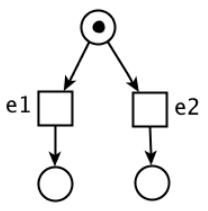
\includegraphics[width=0.75\linewidth]{images/conflitto_avanti.png}
    \caption{Conflitto in avanti.}
    \label{fig:conflitto_avanti}
    \end{marginfigure}

    \begin{marginfigure}[-3cm]
        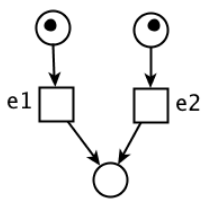
\includegraphics[width=0.75\linewidth]{images/conflitto_indietro.png}
        \caption{Conflitto all'indietro.}
        \label{fig:conflitto_indietro}
    \end{marginfigure}
\end{defn}

\subsubsection{Confusione}
La confusione si presenta in un sistema con conflitti in cui la struttura non permette di stabilire se, nel passaggio da una configurazione $c$ a una configurazione $c'$, è stato risolto un conflitto.

\begin{figure}
    \centering
    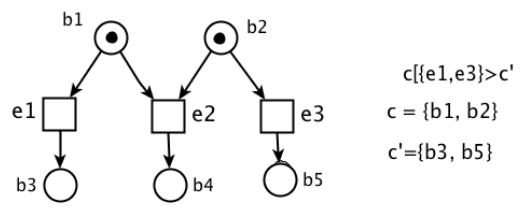
\includegraphics[width=0.5\linewidth]{images/confusione.png}
    \label{fig:confusione}
\end{figure}
In questo sistema non è possibile stabilire se, passando da $c$ a $c'$, sia stato risolto un conflitto tra $e_1$ ed $e_2$ o tra $e_2$ ed $e_3$.

Un altro esempio di confusione si verifica nella mutua esclusione.

\subsubsection{Sequenza}
Siano $\Sigma = (B, E, F, c_{\tn{start}})$ un sistema elementare, $e_1, e_2 \in E$ due eventi e $c \in C_{\Sigma}$ una possibile configurazione di $\Sigma$, $e_1$ ed $e_2$ sono in \textbf{sequenza} in $c$ sse:
\[
    \canFire{c}{e_1}{} \land \lnot \canFire{c}{e_2}{} \land \canFire{\canFire{c}{e_1}{c'}}{e_2}
\]
ovvero $e_2$ può essere eseguito sse prima viene eseguito $e_1$.
C'è quindi una dipendenza causale tra gli eventi $e_1$ ed $e_2$.

\begin{figure}
    \centering
    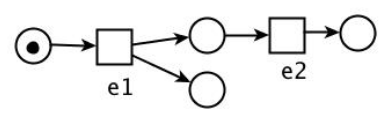
\includegraphics[width=0.5\linewidth]{images/sequenza.png}
    \caption{Due eventi in sequenza.}
    \label{fig:eventi_sequenza}
\end{figure}

\subsubsection{Concorrenza}
Siano $\Sigma = (B, E, F, c_{\tn{start}})$ un sistema elementare, $e_1, e_2 \in E$ due eventi e $c \in C_{\Sigma}$ una possibile configurazione di $\Sigma$, $e_1$ ed $e_2$ sono \textbf{concorrenti} in $c$ sse:
\[
    \canFire{c}{\cbra{e_1, e_2}}{}
\]
ovvero $\cbra{e_1, e_2}$ è un passo abilitato. Questo significa che i due eventi $e_1$ ed $e_2$ sono indipendenti ed entrambi abilitati in $c$.

\begin{figure}
    \centering
    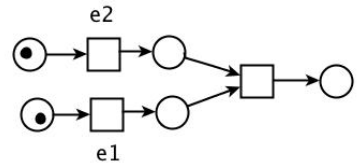
\includegraphics[width=0.5\linewidth]{images/eventi_concorrenti.png}
    \caption{Due eventi concorrenti.}
    \label{fig:eventi_concorrenti}
\end{figure}

\section{Processi non sequenziali e processi ramificati}
Prima di poter spiegare cosa sono i processi non sequenziali e i processi ramificati, è necessario introdurre alcune nozioni.

\subsubsection{Relazioni sugli elementi di una rete}

\begin{defn}
    Sia $N = (B, E, F)$ una rete, la \textbf{relazione di conflitto} $\# \subseteq B \cup E$ specifica quali coppie di elementi della rete $N$ sono causalmente dipendenti da un conflitto in avanti, ed è definita come:
    \[
        x \# y \quad \tn{ sse } \quad \exists e_1, e_2 \in E, (e_1 \neq e_2 \land e_1 \le x \land e_2 \le y) : \preCond{e_1} \cap \preCond{e_2} \neq \emptyset
    \]
\end{defn}

\begin{rem}
    La relazione di conflitto $\#$ è simmetrica ma non transitiva. ???
\end{rem}

\begin{defn}
    La relazione d'ordine parziale largo \footnote{Una relazione d'ordine largo è una relazione riflessiva, simmetrica e transitiva.} $\le \, \subseteq (B \cup E) \times (B \cup E)$ specifica se un elemento è causa di un altro elemento, ed è definita come:
    \[
        \forall x, y \in B \cup E, \quad (x, y) \in \, \le \quad \tn{ sse } \quad x F^*y
    \]
    ovvero è possibile raggiungere $y$ a partire da $x$ usando un numero limitato di transizioni. Se $(x,y) \in \, \le$, allora $x$ \textit{causa} $y$.
    Si può notare che un elemento $x$ causa sè stesso.
\end{defn}

\begin{defn}
    La relazione d'ordine parziale stretto \footnote{Una relazione d'ordine stretto è una relazione riflessiva, antisimmetrica e transitiva.} $< \, \subseteq (B \cup E) \times (B \cup E)$ specifica se un elemento è causa di un altro elemento diverso da sè stesso, ed è definita come:
    \[
        \forall x, y \in B \cup E, \quad (x, y) \in \, < \quad \tn{ sse } \quad x F^*y \land x \neq y
    \]
\end{defn}

\begin{rem}
    $<$ è facilmente ottenibile da $\le$ rimuovendo tutte le coppie della forma $(x,x), \forall x \in B \cup E$.
\end{rem}

\begin{defn}
    La relazione $\tn{li} \subseteq (B \cup E) \times (B \cup E)$ specifica quali elementi della rete sono causalmente dipendenti, ed è definita come: 
    \[
        \forall x, y \in B \cup E, \quad (x, y) \in \tn{ li} \quad \tn{ sse } \quad (x,y) \in \, \le \lor \, (y,x) \in \, \le
    \]
\end{defn}

\begin{defn}
    La relazione $\tn{co} \subseteq (B \cup E) \times (B \cup E)$ specifica quali elementi della rete sono causalmente indipendenti, ed è definita come: 
    \[
        \forall x, y \in B \cup E, \quad (x, y) \in \tn{ co} \quad \tn{ sse } \quad (x,y) \notin \, < \land \, (y,x) \notin \, < \land \, (x,y) \notin \#
    \]
\end{defn}

\begin{rem}
    \begin{align*}
        (x,y) \in \tn{ li } &\longleftrightarrow (y,x) \in \tn{ li}\\
        (x,y) \in \tn{ co } &\longleftrightarrow (y,x) \in \tn{ co}
    \end{align*}
\end{rem}
\begin{rem}
    $\tn{li}$ e $\tn{co}$ sono relazioni riflessive, simmetriche ma non transitive.
\end{rem}
\begin{rem}
    In una rete causale, la relazione $\tn{co}$ non richiede che i due elementi non siano in conflitto in avanti, in quanto ciò è garantito dalla stessa definizione di rete causale.
\end{rem}

\subsubsection{Sottoinsiemi di elementi di una rete}
\begin{defn}
    Siano $N = (B, E, F)$ una rete e $(B \cup E, \le)$ un poset, $C \subseteq B \cup E$ è un \textbf{coset} sse:
    \[
        \forall x, y \in C, x \tn{ co } y
    \]
    ovvero gli elementi di un coset sono tutti causalmente indipendenti tra loro. 
\end{defn}

\begin{rem}
    In un coset, la relazione $\tn{co}$ è transitiva.
\end{rem}

\begin{defn}
    Siano $N = (B, E, F)$ una rete e $(B \cup E, \le)$ un poset, $C \subseteq B \cup E$ è un \textbf{taglio} sse $C$ è un poset massimale, ovvero:
    \[
        C \tn{ è un coset } \, \land \, \forall x \in (B \cup E) \setminus C, \, \exists c \in C : x \tn{ li } c
    \]
    ovvero ogni altro elemento che non appartiene a $C$ è causalmente dipendente da almeno un elemento di $C$, o viceversa.
\end{defn}

\begin{defn}
    Un taglio $C$ è un \textbf{B-taglio} sse $C \subseteq B$, ovvero è formato da soli stati locali.
\end{defn}

\begin{defn}
    Un taglio $C$ è un \textbf{E-taglio} sse $C \subseteq E$, ovvero è formato da soli eventi.
\end{defn}

\begin{rem}
    Tutti gli eventi all'interno di un E-taglio possono essere eseguiti in maniera concorrente. Essendo un E-taglio l'insieme di cardinalità massima $n$ che contiene solo eventi indipendenti tra loro, il sistema necessita di $n$ processori per l'esecuzione in minor tempo possibile degli $n$ eventi.\\
    Il numero di processori per una rete (da cui si deriva la rete di occorrenze), è pari alla cardinalità massima tra le cardinalità degli E-tagli di tutti i processi non sequenziale che è possibile definire.
\end{rem}

\begin{defn}
    Siano $N = (B, E, F)$ una rete e $(B \cup E, \le)$ un poset, $L \subseteq B \cup E$ è un \textbf{liset} sse:
    \[
        \forall x, y \in L, x \tn{ li } y
    \]
    ovvero gli elementi di un liset sono tutti causalmente dipendenti tra loro.
\end{defn}

\begin{rem}
    In un liset, la relazione $\tn{li}$ è transitiva.
\end{rem}

\begin{defn}
    Siano $N = (B, E, F)$ una rete e $(B \cup E, \le)$ un poset, $L \subseteq B \cup E$ è una \textbf{linea} sse è un liset massimale, ovvero:
    \[
        L \tn{ è un coset } \, \land \, \forall x \in (B \cup E) \setminus L, \, \exists l \in L : x \tn{ co } l
    \]
    ovvero ogni altro elemento che non appartiene a $L$ è causalmente indipendente da almeno un elemento di $C$, o viceversa.
\end{defn}



Su una rete di occorrenze è possibile definire le funzioni
\begin{align*}
    \tn{past}: B \cup E &\rightarrow \mathcal{P}(B \cup E)\\
    \tn{future}: B \cup E &\rightarrow \mathcal{P}(B \cup E)
\end{align*}

$\tn{past}$ restituisce tutti gli elementi della rete che causano $x$, mentre $\tn{future}$ restituisce tutti gli elementi che sono causati da $x$.\\
Per definizione di rete di occorrenze, $\tn{past}(x)$ è sicuramente un insieme di cardinalità finita, mentre $\tn{past}(x)$ può avere cardinalità infinita numerabile.

\begin{rem}
    Tutti gli elementi della rete che non appartengono nè a $\tn{past}(x)$ nè a $\tn{future}(x)$ possono essere eseguiti in maniera concorrente rispetto a $x$.
\end{rem}

\subsubsection{Processo ramificato}
\begin{defn}
    Una rete $N = (B, E, F)$ è una \textbf{rete di occorrenze} sse:
    \begin{itemize}
        \item $\forall b \in B, |\preCond{b}| = 1$, ovvero sono accettati solo conflitti in avanti.
        \item $\forall x, y \in B \cup E, (x,y) \in F^+ \rightarrow (y,x) \notin F^+$, ovvero non sono presenti cicli.
        \item $\forall e \in E$, l'insieme $\cbra{x \in B \cup E : x F^*e}$ ha cardinalità finita.
        \item la relazione di conflitto $\#$ è irriflessiva \footnote{E di conseguenza antisimmetrica.}, ovvero un unico elemento non dipendente causalmente da due eventi in conflitto in avanti.
    \end{itemize}
\end{defn}
???

\subsubsection{Processo non sequenziale}
Una rete causale è un tipo particolare di rete di occorrenze, che non presenta alcun conflitto.\\
Una \textbf{rete causale} è una tripla $N = (B, E, F)$ tale che \footnote[][-1cm]{L'ulteriore condizione presente nelle reti di occorrenza, ovvero che la relazione di conflitto sia irriflessiva, collassa nella prima condizione per le reti clausali: non avendo alcun conflitto, per la rete clausale vale $\# = \emptyset$.}:
\begin{itemize}
    \item $\forall b \in B, \lvert \preCond{b} \rvert \le 1 \land \lvert \postCond{b} \rvert \le 1$, ovvero non sono presenti conflitti \footnote[][1cm]{In un conflitto in avanti, lo stato pre-condizione ha due post-eventi. In un conflitto all'indietro, lo stato post-condizione ha due pre-eventi. Di conseguenza, imporre un numero di pre-eventi e post-eventi minore o uguale a uno implica l'assenza di conflitti.};
    \item $\forall x, y \in B \cup E, \quad (x, y) \in F^+ \rightarrow (y, x) \notin F^+$, ovvero non sono presenti cicli;
    \item $\forall e \in E$, la cardinalità dell'insieme $\cbra{x \in B \cup E | x \, F^* e}$ è finita, ovvero i predecessori di un qualsiasi elemento sono in numero finito.
\end{itemize}

\begin{rem}
    Una rete causale ammette elementi isolati, ovvero elementi senza archi in ingresso e archi in uscita.
\end{rem}

Una rete causale rappresenta una delle possibili esecuzioni del sistema concorrente, ovvero un suo processo non sequenziale, non tutte le possibili esecuzioni. La coppia $(N, \phi)$ che definisce un processo non sequenziale è quindi il processo non sequenziale costruito dalla rete $N$ usando la funzione $\phi$. Diversi processi non sequenziali per la stessa rete definiranno la funzione $\phi$ in maniera diversa ($\phi$ deve comunque rispettare tutte le caratteristiche che deve avere la funzione che permette di definire un processo non sequenziale).

Sia $\Sigma = (B, E, F, c_{\tn{start}})$ un sistema elementare senza contatti e finito (e quindi k-densa) \footnote{Con sistema elementare finito si intende un sistema per cui $B \cup E$ è un insieme di cardinalità finita.}.
$\ang{\Sigma, \phi}$ è un \textbf{processo non sequenziale} sse 

???

Un processo non sequenziale finito e senza contatti, allora $N$ è k-densa.

K-DENSIT
Una rete è $k$-densa se, se ogni linea si interseca una singola volta con ogni altro taglio e, viceversa, ogni taglio si interseca una singola volta con ogni altra linea.

Un taglio e una linea si intersecano esattamente in un punto perchè se si incontrassero in più punti, allora tutti i punti di intersezione rappresenterebbero elementi che sono contemporaneamente casualmente dipendenti (li) e casualmente indipendenti (co), violando quindi i tagli e le linee definite.

Una rete finita è sicuramente $k$-densa.




